% Déclaration des titres
% -------------------------------------

\def\discipline{Informatique}
\def\xxtete{Informatique}

\def\classe{\textsf{MPSI}}
\def\xxnumpartie{Sem. 2}
\def\xxpartie{}
\def\xxdate{1 mars 2022}

\def\xxchapitre{Introduction aux graphes}
\def\xxnumchapitre{Ch. 6}
\def\xxnomchapitre{Introduction aux graphes}
\def\xxnumactivite{01}

\def\xxposongletx{2}
\def\xxposonglettext{1.45}
\def\xxposonglety{19}%16

\def\xxonglet{\textsf{S2}}
\def\xxauteur{\textsl{E. Durif -- X. Pessoles \\ J.-P. Berne }}


\def\xxpied{%
\xxnumpartie -- \xxnomchapitre \\
%Cycle \xxnumpartie -- \xxpartie\\
%Chapitre \xxnumchapitre -- \xxactivite -\xxnumactivite -- \xxnomchapitre%
%Chapitre \xxnumchapitre -- 
\xxactivite \xxnumactivite %
}

\setcounter{secnumdepth}{5}
\chapterimage{Fond_GRAPHE}
\def\xxfigures{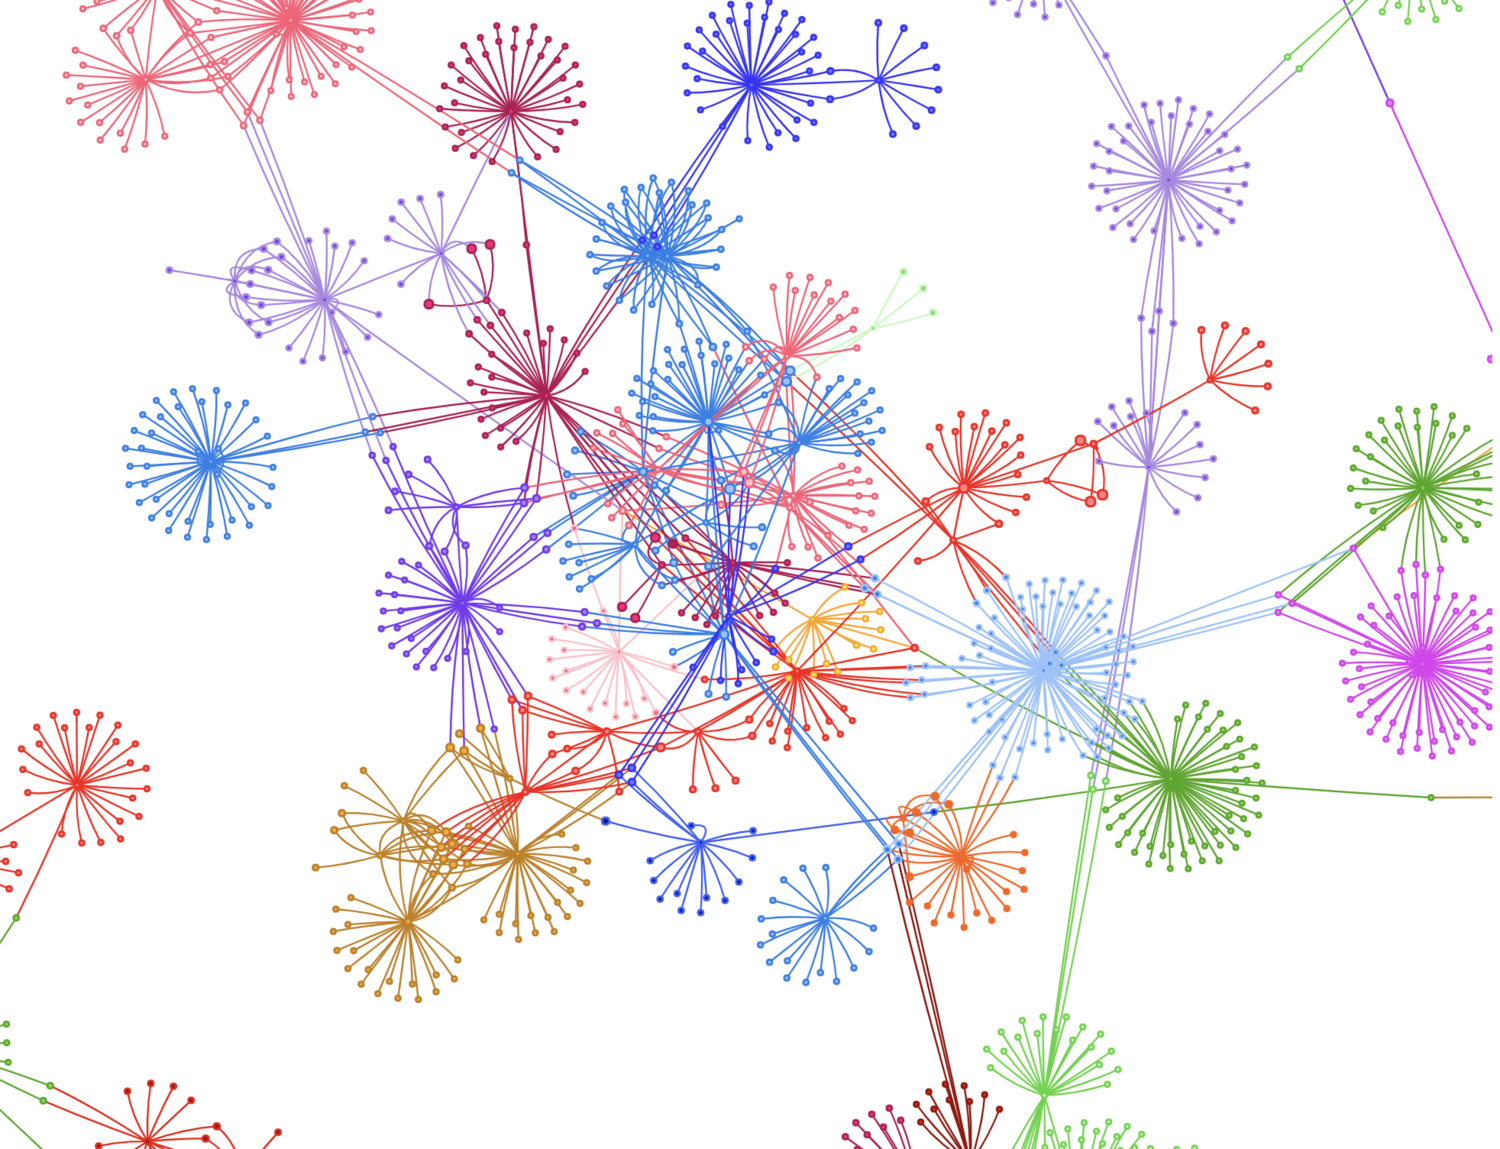
\includegraphics[width=3cm]{graph_cluster_distant}}

\def\xxcompetences{%
\textsl{%
%\vspace{-.5cm}
%\textbf{Savoirs et compétences :}\\
%\vspace{-.1cm}
%\begin{itemize}[label=\ding{112},font=\color{ocre}]
%\item Th. 0 : Connaître les bases de l'algorithmique et de la programmation (variable, types, structures, fonctions).
%\end{itemize}
}}





%---------------------------------------------------------------------------


